% ============================================================
% M3 S3 练习件·W3 臂G 片2 —— 课时19 章末总结与复习＝照抄课时01 母版体例
% 生成：M3 成卷轮 S3 W3 臂G｜2026-09-14｜编译 cwd＝本目录（中文路径禁 \input 绝对路径）
%   xelatex main-true.tex ×2 → 含详解印本；xelatex main-false.tex ×2 → 纯题版（单源双本）
% 输入链（全只读）：题面库 课时19-章末总结与复习.md（题面逐字装配）＋ -答案侧.md（值逐字回嵌）
%   ＋ 定稿/批E-课时19-章末总结与复习.md §七 补产全文区（详解回嵌源）；toolchain＝qp-m3.sty
%   （钉后版 md5 7c3930362be8a0a2bdf21bbf8ac16573，本地挂载副本，破损即停）。
% 母版体例：详见《练习件母版体例说明.md》（课时01）；同波近范模：课时12/18（W3 臂F/臂G）；
%   门谱读数见 过程件 工作区/_tmpM3S3W3臂G0914/。
% 键账：件内 ansblock 键集 ≡ 题面库片练键集 ≡ manifest 练键序 01~16（16 键，零缺漏零多余）；
%   拓区隔离：2章-拓/测/滚 键不入本件（S4 拓展册收）；导学键 2章-导-课时19-G1~G5 属导学件域
%   （G5 补冻 3单选＋2填空），亦不入练习件。
% 卷式例外案B：练习件不属卷式——答案块物理落点恒为题后 ansblock，禁卷末附卷制；
%   全线括线模（导言 \ansblockgrayfalse 一次置定，件内不切换；灰底盒不可跨栏断，练习件禁用）。
% 题序＝manifest 键序 01~16（零重排）；印面题号 1~16 连号（\tihao 号＝\ansitem 号同键）；
%   三档切位 1~7／8~14／15~16（照库序切位，非难度重排）。
% 槽配实录：单选5（01/02/07/09/14）＋多选2（11/12，≤4 合规）＋填空1（10）＋解答8
%   （03~06/08/13/15/16）；10选4填2解 为波次方案基线槽配，本片实配照题面侧头标按实登记
%   （教材复习题A组 6 题＝01~06 形态按源，富矿池 10 题＝07~16，批E §一 满足度同口径）。
% 选项槽位：默认四连排（0.25\linewidth−0.25\lxhang），超宽降档梯 四连排→两连排
%   （0.5\linewidth−0.5\lxhang−0.25em）→单列 \lxopt；禁缩字号/负 kern/删标点凑宽。
%   本片实测降档：题1 单列（长文选项）、题2/9/12/14 两连排、题7 四连排、题11 单列（多选长文）
%   （真算读数见 值台账-课时19.json「降档登记」）。
% 解答书写区：03~06 无小问 16mm×4；08 三问 32mm；13/15/16 两问 24mm×3（16~40mm 带内；
%   纯题档吞 ansblock 不吞 \liubai）。
% 填空印答：题10 \kongda{2}（详解版印答、纯题版退定宽空线，两档等形）。
% 图债：题10（19-10）焦点三角形构形图、题16（19-16）双抛物线构形图已于 0914 印前回冲印面
%   （图资源/19-10.png、19-16.png，重绘图；题面「如图」处 \ansfig 插桩；台账「图债」同账销案）。
% 题面注记（不入印面）：19-03 教材A13 勘误依原文修正（椭圆右半，§三.2 留痕）；19-04/19-06
%   跨件 CP 同族异构并存（衔接节定稿 §五）；19-06 源无选项设问以解答形成卷；19-13 前置闸
%   0913 黄旗⑤ 点差法同族挂注（拓展册件6-19/20 侧归该件责任臂）；19-15 双胞胎取37弃38
%   （查重纪律），(2) 答含退化支「退化但合法」（§三.3）；19-16 交接账「件19-15 答案引用待核」
%   已核销（亲算①-4 全推导，§三.4）。
% 值注记：19-08/19-16（A档0.40）值照亲算档 ①-3/①-4 逐项核对一致；教材A组 6 题值照定稿
%   速算附注（本轮独立推演，A13 依原文修正）；19-16 值含 ASCII 下划线 x_A——导言置文本安全
%   下划线直印（同课时18 方案，值字节照答案侧逐字）。
% ============================================================
\documentclass[fontset=none]{ctexart}
\usepackage{qp-m3}
% —— 印面逐字符号路由补钉（承导学件母版；− 走 TNR、▱ NSC 子块；禁改 sty 保 md5） ——
\xeCJKDeclareCharClass{Default}{"2212}%
\setCJKfamilyfont{nscblk}[Path=C:/提示词/工作区/字替对照-0909/variantF/fonts/,BoldFont=NSC-w600.ttf]{NSC-w500.ttf}%
\xeCJKDeclareSubCJKBlock{nscblk}{"25B1}%
\newcommand{\pxparallelogram}{{\CJKfamily{nscblk}▱}}%
% —— 文本态下划线安全（19-16 值 x_A 直印；数学态仍下标；内核方案，不引包） ——
\begingroup
  \catcode`\_=13 %
  \gdef_{\TextOrMath{\textunderscore}{\sb}}%
\endgroup
\AtBeginDocument{\catcode`\_=13 }%
% —— 断行微调（CJK 胶 0.10em＋拉伸 plus 0.30em，课时16 实证校准 0914：窄栏详解长公式链；
%    \emergencystretch 不另设） ——
\xeCJKsetup{CJKglue={\hskip 0.10em plus 0.30em minus 0.05em}}%
% —— 练习件全线括线模（S3 波次方案 §四.3：导言一次置定、件内不切换） ——
\ansblockgrayfalse
% —— 页脚件名（qp-headfoot 复用入口） ——
\renewcommand{\qpzhangming}{第二章\quad 平面解析几何}%
\renewcommand{\qpjianming}{练习件}%

\begin{document}
%装配轮S6三本跨本连续页码（G7方案B）setcounter 注入位
\setcounter{page}{242}

\keshi{第19课时\quad 章末总结与复习}
\begin{multicols}{2}
\emergencystretch=1em

% ============================================================
% 基础巩固（题1~7＝19-01~07：单选3＋解答4；题后紧跟答案制，全线括线 ansblock）
% ============================================================
\dangbadge{基}{础}{巩}{固}

\tihao{1}\zu{概念辨析（离心率载体）×单选} \tieside{简单(知识点一)}方程\(x^{2}-4x+1=0\)的两个根可分别作为\nobreak(\kongwei)

\lxopt{A．椭圆和双曲线的离心率}

\lxopt{B．两抛物线的离心率}

\lxopt{C．椭圆和抛物线的离心率}

\lxopt{D．两椭圆的离心率}

\begin{ansblock}[2章-练-课时19-01]
% ans:2章-练-课时19-01
\ansitem{1}{A}
\ansnote{详解}{求根公式：\(x=2\pm\sqrt{3}\)，其中\(2-\sqrt{3}\approx 0.27\in(0,1)\)可作椭圆离心率，\(2+\sqrt{3}\approx 3.73\in(1,+\infty)\)可作双曲线离心率。抛物线离心率恒等于1，两根均不为1，排除B、C；两椭圆离心率都须在\((0,1)\)内，而\(2+\sqrt{3}>1\)，排除D。故选：A。}
\end{ansblock}

\tihao{2}\zu{概念辨析（曲线族）×单选} \tieside{简单(知识点一)}曲线\(x^{2}/25+y^{2}/9=1\)与曲线\(x^{2}/(25-k)+y^{2}/(9-k)=1\)（\(k<9\)）的\nobreak(\kongwei)
\bindopt {\fontsize{10.5pt}{\qpTJgLeadLiti}\selectfont \makebox[\dimexpr0.5\linewidth-0.5\lxhang-0.25em\relax][l]{A．长轴长相等}\makebox[\dimexpr0.5\linewidth-0.5\lxhang-0.25em\relax][l]{B．焦距相等}\par}
\bindopt {\fontsize{10.5pt}{\qpTJgLeadLiti}\selectfont \makebox[\dimexpr0.5\linewidth-0.5\lxhang-0.25em\relax][l]{C．离心率相等}\makebox[\dimexpr0.5\linewidth-0.5\lxhang-0.25em\relax][l]{D．短轴长相等}\par}

\begin{ansblock}[2章-练-课时19-02]
% ans:2章-练-课时19-02
\ansitem{2}{B}
\ansnote{详解}{\(k<9\Rightarrow 25-k>9-k>0\)，第二曲线为椭圆，其\(c^{2}=(25-k)-(9-k)=16\)，与\(k\)无关；第一曲线\(c^{2}=25-9=16\)。故两曲线半焦距均为4、焦距均为8，选B。长轴\(10\)与\(2\sqrt{25-k}\)、短轴\(6\)与\(2\sqrt{9-k}\)、离心率\(e^{2}=16/25\)与\(16/(25-k)\)均随\(k\)变动，排除A、C、D。}
\end{ansblock}

\tihao{3}\zu{定义求轨迹×解答} \tieside{中档(知识点一)}已知\(\triangle ABC\)的三边\(AB\)、\(BC\)、\(CA\)满足\(2|BC|=|AB|+|CA|\)，\(|AB|>|CA|\)，且\(B(-1,0)\)、\(C(1,0)\)，求点\(A\)的轨迹方程，并说明它是什么曲线。
\liubai[16mm]{解答书写区}

\begin{ansblock}[2章-练-课时19-03]
% ans:2章-练-课时19-03
\ansitem{3}{x²/4+y²/3=1（x>0，y≠0），椭圆 x²/4+y²/3=1 的右半部分（不含与 x 轴的交点）}
\ansnote{详解}{\(|BC|=2\Rightarrow|AB|+|CA|=2|BC|=4>|BC|=2\)，由椭圆定义，\(A\)的轨迹是以\(B\)、\(C\)为焦点、长半轴\(a=2\)、半焦距\(c=1\)、短半轴\(b^{2}=a^{2}-c^{2}=3\)的椭圆\(x^{2}/4+y^{2}/3=1\)（去掉长轴端点，因\(4>|BC|\)严格成立）。在该椭圆上\(|AB|=a+ex\)、\(|CA|=a-ex\)（\(e=1/2\)），\(|AB|>|CA|\Leftrightarrow x>0\)。又\(A\)为三角形顶点，不能与\(B\)、\(C\)共线\(\Rightarrow y\neq 0\)（舍去点\((2,0)\)）。故轨迹为\(x^{2}/4+y^{2}/3=1\)（\(x>0\)，\(y\neq 0\)），是椭圆的右半（不含顶点）。}
\end{ansblock}

\tihao{4}\zu{含参方程判型×解答} \tieside{中档(知识点一)}若方程\((3-a)x^{2}+(a+1)y^{2}+a^{2}-2a-3=0\)是双曲线的方程，求实数\(a\)的取值范围。
\liubai[16mm]{解答书写区}

\begin{ansblock}[2章-练-课时19-04]
% ans:2章-练-课时19-04
\ansitem{4}{a<−1 或 a>3}
\ansnote{详解}{双曲线型须二次项系数异号：\((3-a)(a+1)<0\Leftrightarrow a<-1\)或\(a>3\)。此时常数项\(a^{2}-2a-3=(a-3)(a+1)>0\)自动相容，方程确为双曲线：\(a>3\)时移项配方得\(x^{2}/(a+1)-y^{2}/(a-3)=1\)；\(a<-1\)时同法得\(x^{2}/(a+1)-y^{2}/(a-3)=1\)（分子分母同乘\(-1\)后仍为平方差形式）。即\(-1<a<3\)时为椭圆型或虚轨迹/退化，不取。故\(a\in(-\infty,-1)\cup(3,+\infty)\)。}
\end{ansblock}

\tihao{5}\zu{位置关系定参×解答} \tieside{中档(知识点二)}已知直线\(y=kx+2\)与椭圆\(x^{2}+2y^{2}=2\)相交于不同的两点，求\(k\)的取值范围。
\liubai[16mm]{解答书写区}

\begin{ansblock}[2章-练-课时19-05]
% ans:2章-练-课时19-05
\ansitem{5}{k<−√6/2 或 k>√6/2}
\ansnote{详解}{联立消\(y\)：\((1+2k^{2})x^{2}+8kx+6=0\)。相交于不同两点\(\Leftrightarrow\Delta>0\)：\(\Delta=64k^{2}-24(1+2k^{2})=16k^{2}-24=8(2k^{2}-3)>0\Leftrightarrow k^{2}>3/2\Leftrightarrow|k|>\sqrt{6}/2\)。故\(k<-\sqrt{6}/2\)或\(k>\sqrt{6}/2\)。}
\end{ansblock}

\tihao{6}\zu{公共点分类×解答} \tieside{简单(知识点二)}直线\(l\)过点\(P(2,4)\)且与抛物线\(y^{2}=8x\)只有一个公共点，求直线\(l\)的方程。
\liubai[16mm]{解答书写区}

\begin{ansblock}[2章-练-课时19-06]
% ans:2章-练-课时19-06
\ansitem{6}{y=4 或 y=x+2}
\ansnote{详解}{①斜率不存在：\(x=2\)代入\(y^{2}=16\)得两点\((2,\pm 4)\)，不合，舍。②斜率\(k=0\)：\(y=4\)，与抛物线恰一公共点\((2,4)\)，合。③\(k\neq 0\)：设\(y-4=k(x-2)\)，以\(x=y^{2}/8\)代入并整理：\(ky^{2}-8y+32-16k=0\)，恰一公共点\(\Leftrightarrow\Delta=64-4k(32-16k)=64(k-1)^{2}=0\Rightarrow k=1\Rightarrow y=x+2\)。综上共两条：\(y=4\)与\(y=x+2\)。}
\end{ansblock}

\tihao{7}\zu{方程直求×单选} \tieside{中档(知识点一)}双曲线\(C\)：\(x^{2}/a^{2}-y^{2}/b^{2}=1\)（\(a>0\)，\(b>0\)）的离心率为\(\sqrt{2}\)，抛物线\(y^{2}=2px\)（\(p>0\)）的准线与双曲线\(C\)的渐近线交于\(A\)、\(B\)点，\(\triangle OAB\)（\(O\)为坐标原点）的面积为4，则抛物线的方程为\nobreak(\kongwei)
\bindopt {\fontsize{10.5pt}{\qpTJgLeadLiti}\selectfont \makebox[\dimexpr0.5\linewidth-0.5\lxhang-0.25em\relax][l]{A．\(y^{2}=4x\)}\makebox[\dimexpr0.5\linewidth-0.5\lxhang-0.25em\relax][l]{B．\(y^{2}=6x\)}\par}
\bindopt {\fontsize{10.5pt}{\qpTJgLeadLiti}\selectfont \makebox[\dimexpr0.5\linewidth-0.5\lxhang-0.25em\relax][l]{C．\(y^{2}=8x\)}\makebox[\dimexpr0.5\linewidth-0.5\lxhang-0.25em\relax][l]{D．\(y^{2}=16x\)}\par}

\begin{ansblock}[2章-练-课时19-07]
% ans:2章-练-课时19-07
\ansitem{7}{C}
\ansnote{详解}{\(e=\sqrt{2}\Rightarrow a=b\Rightarrow\)等轴双曲线\(\Rightarrow\)渐近线\(y=\pm x\)。准线\(x=-p/2\)，交渐近线于\(A(-p/2,p/2)\)、\(B(-p/2,-p/2)\)，\(|AB|=p\)，\(O\)到\(AB\)距离\(p/2\)，故\(S=(1/2)\cdot p\cdot p/2=p^{2}/4=4\Rightarrow p=4\Rightarrow y^{2}=8x\)。故选：C。}
\end{ansblock}

% ============================================================
% 综合提升（题8~14＝19-08~14：解答2＋单选1＋填空1＋多选2＋单选1＋解答1）
% ============================================================
\dangbadge{综}{合}{提}{升}

\tihao{8}\zu{方程直求压轴×解答} \tieside{难(知识点二)}已知双曲线\(\Gamma\)：\(x^{2}-y^{2}=4\)，双曲线\(\Gamma\)的右焦点为\(F\)，圆\(C\)的圆心在\(y\)轴正半轴上，且经过坐标原点\(O\)，圆\(C\)与双曲线\(\Gamma\)的右支交于\(A\)、\(B\)两点。(1) 当\(\triangle OFA\)是以\(F\)为直角顶点的直角三角形，求\(\triangle OFA\)的面积；(2) 若点\(A\)的坐标是\((\sqrt{5},1)\)，求直线\(AB\)的方程；(3) 求证：直线\(AB\)与圆\(x^{2}+y^{2}=2\)相切。
\liubai[32mm]{解答书写区}

\begin{ansblock}[2章-练-课时19-08]
% ans:2章-练-课时19-08
\ansitem{8}{(1) 2√2；(2) y=[(2√2+√5)/3]x−(2√10+2)/3；(3) 证毕（O 到 AB 距离恒为 √2）}
\ansnote{详解}{\(c^{2}=4+4=8\)，即\(F(2\sqrt{2},0)\)。圆心\((0,m)\)（\(m>0\)）、过\(O\)，即半径\(m\)：\(x^{2}+y^{2}-2my=0\)。\par\noindent (1) \(AF\perp OF\)（\(x\)轴），即\(x_A=2\sqrt{2}\)，得\(y_A^{2}=8-4=4\)，取\(A(2\sqrt{2},2)\)，\(S=(1/2)\cdot|OF|\cdot|y_A|=(1/2)\cdot 2\sqrt{2}\cdot 2=2\sqrt{2}\)。\par\noindent (2) 代\(A(\sqrt{5},1)\)：\(5+1-2m=0\)，得\(m=3\)。圆与\(\Gamma\)联立（\(x^{2}-y^{2}=4\)、\(x^{2}+y^{2}-6y=0\)相减）得\(y^{2}-3y+2=0\)，即\(y=1\)（\(A\)）或\(y=2\)，得\(B(2\sqrt{2},2)\)。\(k_{AB}=(2-1)/(2\sqrt{2}-\sqrt{5})=(2\sqrt{2}+\sqrt{5})/3\)（分母有理化，\((2\sqrt{2})^{2}-(\sqrt{5})^{2}=3\)）；截距\(=1-k\sqrt{5}=1-(2\sqrt{10}+5)/3=-(2\sqrt{10}+2)/3\)，直线\(AB\)同值。\par\noindent (3) 一般情形：圆\(x^{2}+y^{2}-2my=0\)与\(\Gamma\)消\(x\)得\(y^{2}-my+2=0\)，即\(y_1y_2=2\)、\(y_1^{2}+y_2^{2}=m^{2}-4\)；右支\(x_i=\sqrt{y_i^{2}+4}\)，得\(x_1x_2=\sqrt{(y_1y_2)^{2}+4(y_1^{2}+y_2^{2})+16}=2\sqrt{m^{2}+1}\)、\(x_1^{2}+x_2^{2}=m^{2}+4\)。原点到\(AB\)的距离\(d=|x_1y_2-x_2y_1|/|AB|\)，其中分子平方\(=x_1^{2}y_2^{2}+x_2^{2}y_1^{2}-2x_1x_2y_1y_2=y_2^{2}(y_1^{2}+4)+y_1^{2}(y_2^{2}+4)-4\sqrt{m^{2}+1}\cdot 2=2(y_1y_2)^{2}+4(y_1^{2}+y_2^{2})-8\sqrt{m^{2}+1}=4m^{2}-8-8\sqrt{m^{2}+1}\)；分母平方\(=(x_1^{2}+x_2^{2}-2x_1x_2)+(y_1^{2}+y_2^{2}-2y_1y_2)=(m^{2}+4-4\sqrt{m^{2}+1})+(m^{2}-4-4)=2m^{2}-4-4\sqrt{m^{2}+1}\)。分子平方\(=2\times\)分母平方恒成立（\(m>2\sqrt{2}\)时分母\(>0\)），即\(d^{2}\equiv 2\)，\(d=\sqrt{2}=\)圆\(x^{2}+y^{2}=2\)的半径，故相切，证毕。}
\end{ansblock}

\tihao{9}\zu{离心率约束×单选} \tieside{中档(知识点一)}设\(F_1\)、\(F_2\)是椭圆\(C_1\)：\(x^{2}/a_1^{2}+y^{2}/b_1^{2}=1\)（\(a_1>b_1>0\)）与双曲线\(C_2\)：\(x^{2}/a_2^{2}-y^{2}/b_2^{2}=1\)（\(a_2>0\)，\(b_2>0\)）的公共焦点，曲线\(C_1\)、\(C_2\)在第一象限内交于点\(M\)，\(\angle F_1MF_2=90^{\circ}\)。若椭圆的离心率\(e_1\in[\sqrt{6}/3,1)\)，则双曲线的离心率\(e_2\)的范围是\nobreak(\kongwei)
\bindopt {\fontsize{10.5pt}{\qpTJgLeadLiti}\selectfont \makebox[\dimexpr0.5\linewidth-0.5\lxhang-0.25em\relax][l]{A．\((1,\sqrt{2}]\)}\makebox[\dimexpr0.5\linewidth-0.5\lxhang-0.25em\relax][l]{B．\((1,\sqrt{3}]\)}\par}
\bindopt {\fontsize{10.5pt}{\qpTJgLeadLiti}\selectfont \makebox[\dimexpr0.5\linewidth-0.5\lxhang-0.25em\relax][l]{C．\([\sqrt{3},+\infty)\)}\makebox[\dimexpr0.5\linewidth-0.5\lxhang-0.25em\relax][l]{D．\([\sqrt{2},+\infty)\)}\par}

\begin{ansblock}[2章-练-课时19-09]
% ans:2章-练-课时19-09
\ansitem{9}{A}
\ansnote{详解}{设\(|MF_1|>|MF_2|\)，则\(|MF_1|+|MF_2|=2a_1\)、\(|MF_1|-|MF_2|=2a_2\)，得\(|MF_1|=a_1+a_2\)、\(|MF_2|=a_1-a_2\)。\(\angle F_1MF_2=90^{\circ}\Rightarrow|MF_1|^{2}+|MF_2|^{2}=4c^{2}\)，即\((a_1+a_2)^{2}+(a_1-a_2)^{2}=4c^{2}\)，得\(a_1^{2}+a_2^{2}=2c^{2}\)，同除\(c^{2}\)：\(1/e_1^{2}+1/e_2^{2}=2\)。\(e_1\in[\sqrt{6}/3,1)\)，即\(1/e_1^{2}\in(1,3/2]\)，得\(1/e_2^{2}=2-1/e_1^{2}\in[1/2,1)\)，即\(e_2^{2}\in(1,2]\)，\(e_2\in(1,\sqrt{2}]\)。故选：A。}
\end{ansblock}

\tihao{10}\zu{离心率约束×填空} \tieside{中档(知识点一)}如图，\(F_1\)、\(F_2\)是椭圆\(C_1\)与双曲线\(C_2\)的公共焦点，\(A\)、\(B\)分别是\(C_1\)、\(C_2\)在第二、四象限的公共点，若\(|OF_1|=|AB|/2\)，且\(\angle OF_1B=\pi/6\)，则\(C_1\)与\(C_2\)的离心率之积为\kongda{2}．
\ansfig{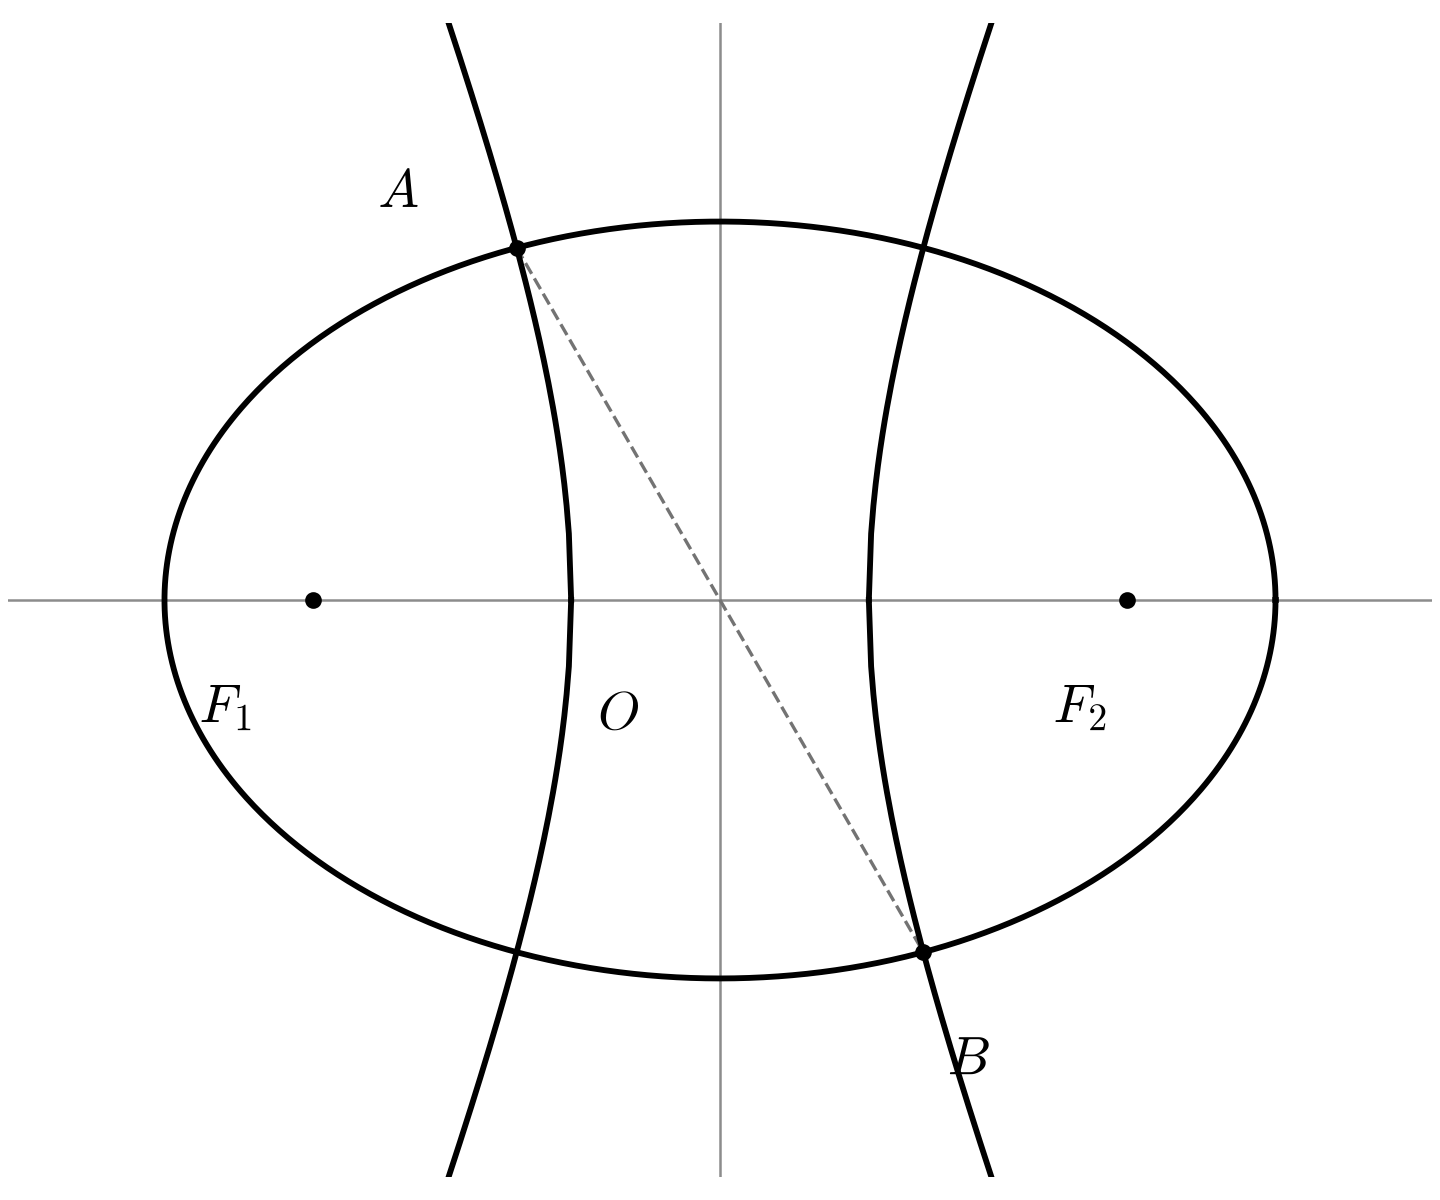
\includegraphics[width=36mm]{figs/19-10.png}}

\begin{ansblock}[2章-练-课时19-10]
% ans:2章-练-课时19-10
\ansitem{10}{2}
\ansnote{详解}{两曲线关于原点对称，即\(O\)为\(AB\)中点，四边形\(AF_1BF_2\)为平行四边形，其对角线\(|AB|=2|OF_1|=2c\)与\(|F_1F_2|=2c\)相等，故四边形为矩形，\(\angle F_1AF_2=\angle F_1BF_2=90^{\circ}\)。\(\triangle OF_1B\)中\(|OF_1|=|OB|=c\)，\(\angle OF_1B=\pi/6\)，顶角\(\angle F_1OB=2\pi/3\)；由\(A=-B\)得\(\angle F_1OA=\pi-2\pi/3=\pi/3\)，而\(|OA|=|OF_1|=c\)，\(\triangle AOF_1\)等边，即\(|AF_1|=c\)且\(\angle AF_1O=\pi/3\)，\(\angle AF_1B=\pi/3+\pi/6=\pi/2\)（与矩形一致）。于是\(|BF_1|=\sqrt{|AB|^{2}-|AF_1|^{2}}=\sqrt{4c^{2}-c^{2}}=\sqrt{3}c\)，且平行四边形对边\(|AF_2|=|BF_1|=\sqrt{3}c\)。椭圆定义：\(c+\sqrt{3}c=2a_1\)，即\(e_1=2/(\sqrt{3}+1)\)；双曲线定义：\(\sqrt{3}c-c=2a_2\)，即\(e_2=2/(\sqrt{3}-1)\)。\(e_1e_2=4/[(\sqrt{3}+1)(\sqrt{3}-1)]=4/2=2\)。}
\end{ansblock}

\tihao{11}\duoxuan\hspace{0.6em}\zu{曲线族判断×多选} \tieside{中档(知识点一)}曲线\(C\)的方程为\(x^{2}/(16+\lambda)+y^{2}/(9+\lambda)=1\)，则下列说法正确的是\nobreak(\kongwei)

\lxopt{A．存在实数\(\lambda\)使得曲线\(C\)的轨迹为圆}

\lxopt{B．存在实数\(\lambda\)使得曲线\(C\)的轨迹为椭圆}

\lxopt{C．存在实数\(\lambda\)使得曲线\(C\)的轨迹为双曲线}

\lxopt{D．无论\(\lambda\)（\(\lambda>-16\)且\(\lambda\neq -9\)）取何值，曲线\(C\)的焦距为定值}

\begin{ansblock}[2章-练-课时19-11]
% ans:2章-练-课时19-11
\ansitem{11}{BCD}
\ansnote{详解}{A：圆须\(16+\lambda=9+\lambda\)，矛盾，不存在，A错。B：\(\lambda>-9\)时\(16+\lambda>9+\lambda>0\)，方程表示焦点在\(x\)轴的椭圆，B对。C：\(-16<\lambda<-9\)时\((16+\lambda)(9+\lambda)<0\)，表示焦点在\(x\)轴的双曲线，C对。D：\(\lambda>-9\)时椭圆\(c^{2}=(16+\lambda)-(9+\lambda)=7\)；\(-16<\lambda<-9\)时双曲线\(c^{2}=(16+\lambda)+[-(9+\lambda)]=7\)，焦距恒为\(2\sqrt{7}\)，D对。故选：BCD。}
\end{ansblock}

\tihao{12}\duoxuan\hspace{0.6em}\zu{共焦点张角×多选} \tieside{中档(知识点一)}已知椭圆\(C_1\)：\(x^{2}/a^{2}+y^{2}/b^{2}=1\)（\(a>b>0\)）的左、右焦点分别为\(F_1\)、\(F_2\)，离心率为\(e_1\)，椭圆\(C_1\)的上顶点为\(M\)，且\(\overrightarrow{MF_1}\cdot\overrightarrow{MF_2}=0\)，双曲线\(C_2\)和椭圆\(C_1\)有相同的焦点，且双曲线\(C_2\)的离心率为\(e_2\)，\(P\)为曲线\(C_1\)与\(C_2\)的一个公共点。若\(\angle F_1PF_2=\pi/3\)，则\nobreak(\kongwei)
\bindopt {\fontsize{10.5pt}{\qpTJgLeadLiti}\selectfont \makebox[\dimexpr0.5\linewidth-0.5\lxhang-0.25em\relax][l]{A．\(e_2/e_1=2\)}\makebox[\dimexpr0.5\linewidth-0.5\lxhang-0.25em\relax][l]{B．\(e_1e_2=\sqrt{3}/2\)}\par}
\bindopt {\fontsize{10.5pt}{\qpTJgLeadLiti}\selectfont \makebox[\dimexpr0.5\linewidth-0.5\lxhang-0.25em\relax][l]{C．\(e_1^{2}+e_2^{2}=5/2\)}\makebox[\dimexpr0.5\linewidth-0.5\lxhang-0.25em\relax][l]{D．\(e_2^{2}-e_1^{2}=1\)}\par}

\begin{ansblock}[2章-练-课时19-12]
% ans:2章-练-课时19-12
\ansitem{12}{BD}
\ansnote{详解}{\(\overrightarrow{MF_1}\cdot\overrightarrow{MF_2}=0\)且\(|MF_1|=|MF_2|=\sqrt{b^{2}+c^{2}}\)，即\(\triangle MF_1F_2\)等腰直角，得\(b=c\)，\(e_1^{2}=b^{2}/(b^{2}+c^{2})=1/2\)，\(e_1=\sqrt{2}/2\)，且\(a=\sqrt{2}c\)。在焦点三角形\(\triangle PF_1F_2\)中\(\angle F_1PF_2=\pi/3\)，设\(|PF_1|=m\)、\(|PF_2|=n\)（\(m>n\)，\(P\)取双曲线右支），则\(m+n=2a_1=2\sqrt{2}c\)、\(m-n=2a_2\)。余弦定理：\(4c^{2}=m^{2}+n^{2}-2mn\cos(\pi/3)=(m+n)^{2}-3mn\)，得\(mn=(8c^{2}-4c^{2})/3=4c^{2}/3\)。故\((m-n)^{2}=(m+n)^{2}-4mn=8c^{2}-16c^{2}/3=8c^{2}/3\)，即\(4a_2^{2}=8c^{2}/3\)，\(a_2^{2}=2c^{2}/3\)，\(e_2^{2}=3/2\)，\(e_2=\sqrt{6}/2\)。逐项：\(e_1e_2=(\sqrt{2}/2)\cdot(\sqrt{6}/2)=\sqrt{3}/2\)，B对；\(e_2^{2}-e_1^{2}=3/2-1/2=1\)，D对；\(e_2/e_1=\sqrt{3}\neq 2\)，A错；\(e_1^{2}+e_2^{2}=2\neq 5/2\)，C错。故选：BD。}
\end{ansblock}

\tihao{13}\zu{中点弦×解答} \tieside{中档(知识点二)}已知双曲线\(C\)：\(x^{2}/a^{2}-y^{2}/b^{2}=1\)（\(a>0\)，\(b>0\)）与椭圆\(x^{2}/18+y^{2}/14=1\)有共同的焦点，点\(A(3,\sqrt{7})\)在双曲线\(C\)上。(1) 求双曲线\(C\)的方程及渐近线方程；(2) 以\(P(1,2)\)为中点作双曲线\(C\)的一条弦\(AB\)，求弦\(AB\)所在直线的方程。
\liubai[24mm]{解答书写区}

\begin{ansblock}[2章-练-课时19-13]
% ans:2章-练-课时19-13
\ansitem{13}{(1) x²/2−y²/2=1、y=±x；(2) x−2y+3=0}
\ansnote{详解}{(1) 椭圆\(c^{2}=18-14=4\)，即双曲线\(c=2\)、\(a^{2}+b^{2}=4\)；\(A\)代入：\(9/a^{2}-7/b^{2}=1\)。令\(u=a^{2}\)：\(9/u-7/(4-u)=1\)，即\(9(4-u)-7u=u(4-u)\)，\(u^{2}-20u+36=0\)，得\(u=2\)或\(u=18\)（\(>c^{2}\)舍），故\(a^{2}=b^{2}=2\)，\(x^{2}/2-y^{2}/2=1\)，渐近线\(y=\pm x\)（等轴双曲线）。\par\noindent (2) 点差法：\(x_1^{2}-y_1^{2}=2\)、\(x_2^{2}-y_2^{2}=2\)相减得\((x_1+x_2)(x_1-x_2)=(y_1+y_2)(y_1-y_2)\)，即\(k_{AB}=(y_1-y_2)/(x_1-x_2)=(x_1+x_2)/(y_1+y_2)=2/4=1/2\)，直线\(y-2=(1/2)(x-1)\)，即\(x-2y+3=0\)。回验：联立消\(y\)得\(3x^{2}-6x-17=0\)，\(\Delta=36+204=240>0\)，为真弦。}
\end{ansblock}

\tihao{14}\zu{文化·黄金分割×单选} \tieside{中档(知识点一)}黄金分割起源于公元前6世纪古希腊的毕达哥拉斯学派，公元前4世纪，古希腊数学家欧多克索斯第一个系统研究了这一问题，公元前300年前后欧几里得撰写《几何原本》时吸收了欧多克索斯的研究成果，进一步系统论述了黄金分割，成为最早的有关黄金分割的论著。黄金分割是指将整体一分为二，较大部分与整体部分的比值等于较小部分与较大部分的比值，其比值为\((\sqrt{5}-1)/2\)，把\((\sqrt{5}-1)/2\)称为黄金分割数。已知双曲线\(x^{2}/(\sqrt{5}-1)^{2}-y^{2}/m=1\)的实轴长与焦距的比值恰好是黄金分割数，则\(m\)的值为\nobreak(\kongwei)
\bindopt {\fontsize{10.5pt}{\qpTJgLeadLiti}\selectfont \makebox[\dimexpr0.5\linewidth-0.5\lxhang-0.25em\relax][l]{A．\(2\sqrt{5}-2\)}\makebox[\dimexpr0.5\linewidth-0.5\lxhang-0.25em\relax][l]{B．\(\sqrt{5}+1\)}\par}
\bindopt {\fontsize{10.5pt}{\qpTJgLeadLiti}\selectfont \makebox[\dimexpr0.5\linewidth-0.5\lxhang-0.25em\relax][l]{C．\(2\)}\makebox[\dimexpr0.5\linewidth-0.5\lxhang-0.25em\relax][l]{D．\(2\sqrt{5}\)}\par}

\begin{ansblock}[2章-练-课时19-14]
% ans:2章-练-课时19-14
\ansitem{14}{A}
\ansnote{详解}{\(a^{2}=(\sqrt{5}-1)^{2}=6-2\sqrt{5}\)。\(a/c=(\sqrt{5}-1)/2\)，即\(c=2a/(\sqrt{5}-1)=a(\sqrt{5}+1)/2\)，得\(c^{2}=a^{2}(3+\sqrt{5})/2\)。\(m=c^{2}-a^{2}=a^{2}[(3+\sqrt{5})/2-1]=a^{2}(1+\sqrt{5})/2=(6-2\sqrt{5})(\sqrt{5}+1)/2=(3-\sqrt{5})(\sqrt{5}+1)=3\sqrt{5}+3-5-\sqrt{5}=2\sqrt{5}-2\)。故选：A。}
\end{ansblock}

% ============================================================
% 思维探索（题15~16＝19-15~16：解答2）
% ============================================================
\dangbadge{思}{维}{探}{索}

\tihao{15}\zu{条件选择×解答} \tieside{中档(知识点一)}在①左顶点为\((-3,0)\)，②双曲线过点\((3\sqrt{2},4)\)，③离心率\(e=5/3\)这三个条件中任选一个，补充在下面问题中并作答（注：如果选择多个条件分别解答，按第一个解答计分）。问题：已知双曲线与椭圆\(x^{2}/49+y^{2}/24=1\)共焦点，且\kongbai{}。(1) 求双曲线的方程；(2) 若点\(P\)在双曲线上，且\(|PF_1|=8\)，求\(|PF_2|\)。
\liubai[24mm]{解答书写区}

\begin{ansblock}[2章-练-课时19-15]
% ans:2章-练-课时19-15
\ansitem{15}{(1) 三条件均得 x²/9−y²/16=1；(2) |PF₂|=2 或 14}
\ansnote{详解}{(1) \(c^{2}=49-24=25\)，即\(c=5\)。选①：左顶点\((-3,0)\)，即\(a=3\)。选②：\(18/a^{2}-16/b^{2}=1\)配\(a^{2}+b^{2}=25\)，即\(18(25-a^{2})-16a^{2}=a^{2}(25-a^{2})\)，\(a^{4}-59a^{2}+450=0\)，得\(a^{2}=9\)或\(50\)（\(>25\)舍），即\(a^{2}=9\)。选③：\(e=c/a=5/3\)，即\(5/a=5/3\)，\(a=3\)。三路均得\(b^{2}=25-9=16\)，双曲线\(x^{2}/9-y^{2}/16=1\)。\par\noindent (2) \(||PF_1|-|PF_2||=2a=6\)，即\(|PF_2|=2\)或\(14\)，均须回验：\(|PF_2|=2\)时\(P\)为右顶点\((3,0)\)（\(|PF_1|=3+5=8\)，\(8-2=6\)合定义——\(P\)、\(F\)成线段，退化但合法）；\(|PF_2|=14\)时\(P\)在左支（\(x=-33/5\)，\(|PF_1|=8\)、\(14-8=6\)，且\(8+14=22>2c=20\)三角形存在）。故\(|PF_2|=2\)或\(14\)。}
\end{ansblock}

\tihao{16}\zu{双抛物线综合×解答} \tieside{难(知识点二)}如图所示，曲线\(C_1\)：\(y^{2}=2p_1x\)（\(p_1>0\)），曲线\(C_2\)：\(y^{2}=-2px\)（\(p>0\)），过点\(C(-1,0)\)作直线交曲线\(C_1\)于点\(A\)，交曲线\(C_2\)于点\(B\)，若点\(C\)在曲线\(C_1\)的准线上。(1) 求\(p_1\)；(2) 若存在直线使点\(B\)为\(AC\)中点，求\(A\)点横坐标（用\(p\)表示）及\(AC\)斜率的范围。
\ansfig{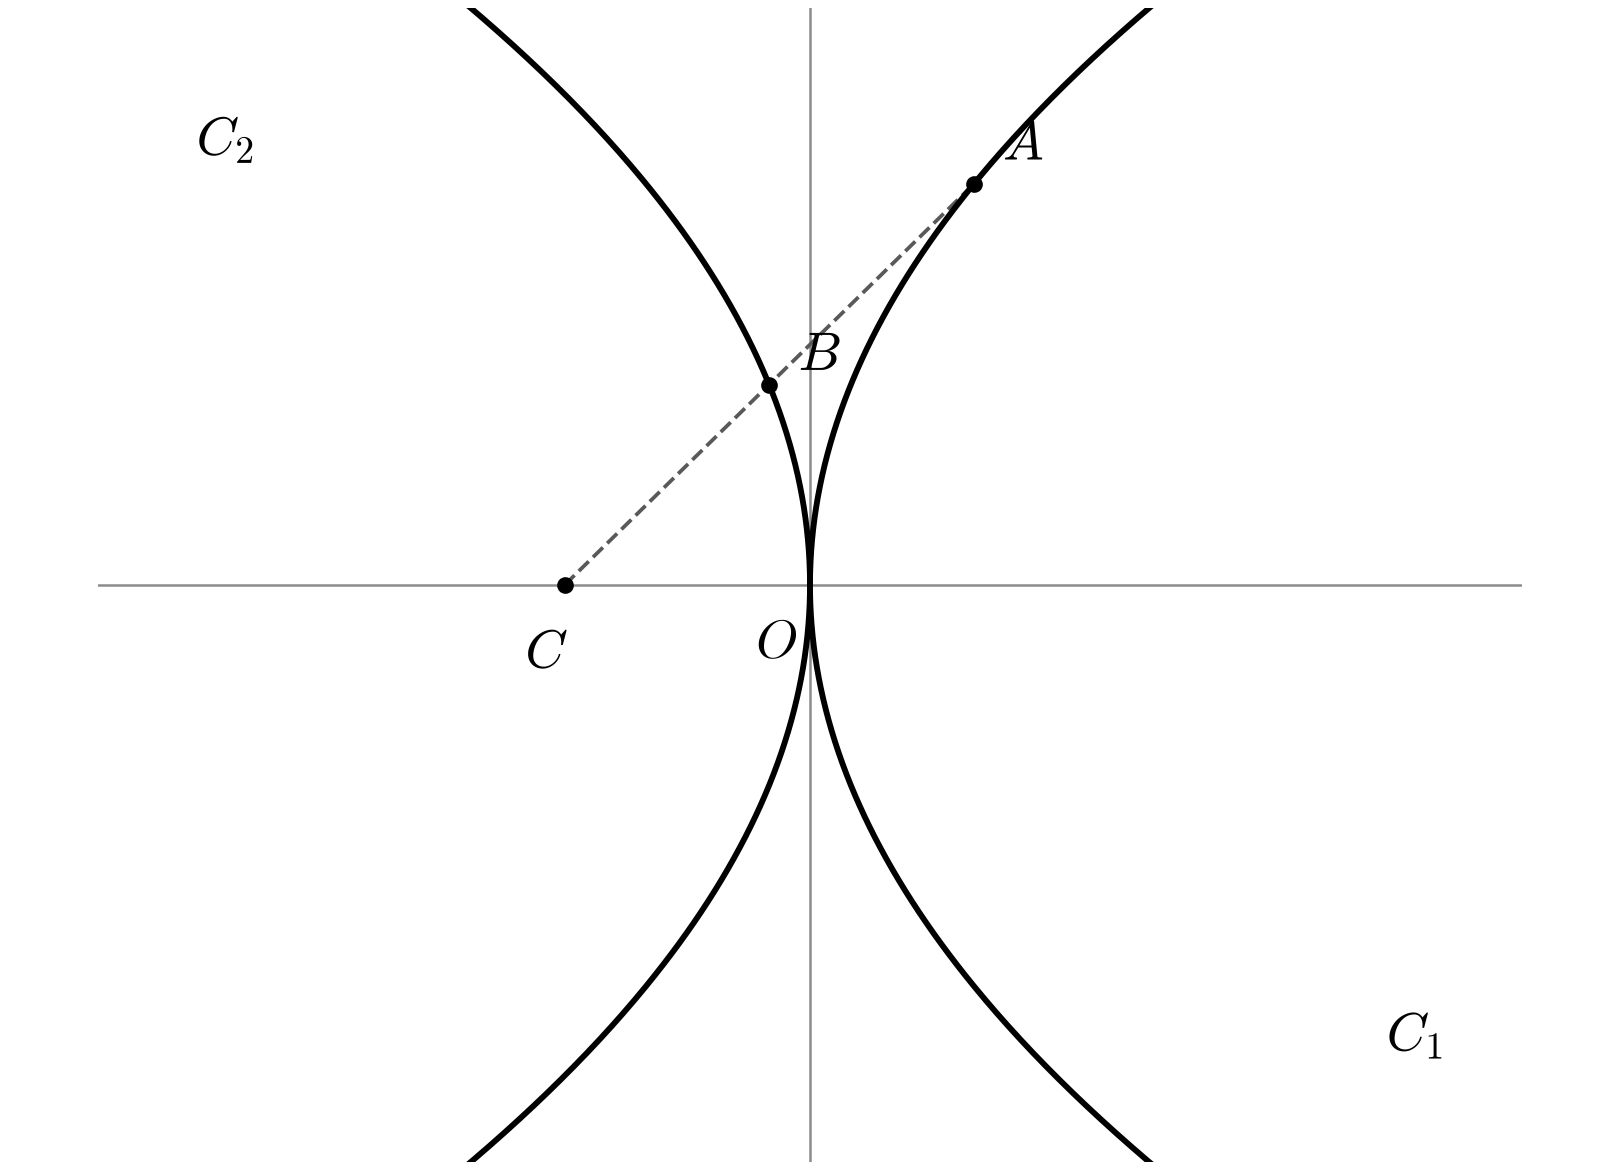
\includegraphics[width=36mm]{figs/19-16.png}}
\liubai[24mm]{解答书写区}

\begin{ansblock}[2章-练-课时19-16]
% ans:2章-练-课时19-16
\ansitem{16}{(1) p₁=2；(2) x_A=p/(p+1)，斜率范围 (−1,0)∪(0,1)}
\ansnote{详解}{(1) \(C_1\)的准线\(x=-p_1/2=-1\)，得\(p_1=2\)，即\(C_1\)：\(y^{2}=4x\)。\par\noindent (2) 设\(B(-t^{2}/(2p),t)\)（\(C_2\)上的参数点），\(B\)为\(AC\)中点、\(C(-1,0)\)，则\(A=2B-C=(1-t^{2}/p,2t)\)。\(A\)在\(C_1\)上：\(4t^{2}=4(1-t^{2}/p)\)，得\(t^{2}=p/(p+1)\in(0,1)\)（\(p>0\)），\(A\)的横坐标\(x_A=1-t^{2}/p=1-1/(p+1)=p/(p+1)\)（\(0<x_A<1\)）。斜率：\(k_{AC}=k_{BC}=t/[-t^{2}/(2p)+1]\)；由\(t^{2}=p/(p+1)\)得\(1/p=1/t^{2}-1\)，故分母\(=-(t^{2}/2)(1/t^{2}-1)+1=(1+t^{2})/2\)，即\(k=2t/(1+t^{2})\)（\(t\neq 0\)，否则\(A=C\)不成弦）。\(k^{2}=4t^{2}/(1+t^{2})^{2}\)，由\(0<t^{2}<1\)得\(0<k^{2}<1\)（等号\(t^{2}=1\)不可达），即\(k\in(-1,0)\cup(0,1)\)，证毕。}
\end{ansblock}

% ---- 尾块（\tailfill 置 \end{multicols} 前；无参＝内容尾随框，每件恰 1 处） ----
\tailfill

\end{multicols}
\end{document}
